%!TEX root = paper.tex

\section{Wrapping Web Services}
\label{sec:wrapping_web_services}

In our approach, wrapping web services is done in two steps: a first step is in charge of the construction of a service request and a second step analyses the response received from the execution of the service, allowing the analysis of response data and the mapping to domain-specific concepts. From this input, we generate JavaScript code to be embedded into web gadgets. This JavaScript code takes query parameters, constructs the service request, analyses the service response and returns result data in the desired format. 

\subsection{Constructing Service Requests} % (fold)
\label{sub:constructing_service_requests}

In this paper we illustrate the interaction with services on simple GET requests as supported e.g. by REST services. Support for other services like POST based services is under construction. In case of a simple GET request, a service request is assembled using a certain URL and a set of parameters. (A POST request would have a text block to be posted. In addition, other header data may be needed to transfer e.g. session ids). As an example, the Ebay Shopping web service will be studied. As documented on the corresponding web site, the following URL is invoked to retrieve a list of items corresponding to the search keywords \emph{USB}:

\begin{listing}
\begin{verbatim}
http://open.api.sandbox.ebay.com/shopping?
  appid=KasselUn-efea-4b93-9505-5dc2ef1ceecd&
  version=517&callname=FindItems&
  ItemSort=EndTime&QueryKeywords=USB&
  responseencoding=XML
\end{verbatim}
\end{listing}

As you may see, the URL invoked is \url{http://open.api.sandbox.ebay.com/shopping} and the parameters used in the example are:
\begin{description}
	\item[appid] this is the application ID obtained to use the API.
	\item[version] the API version.
	\item[callname] in this case \emph{FindItems} to search through all items in Ebay.
	\item[ItemSort] sorting method for the list of items.
	\item[QueryKeywords] list of keywords.
	\item[responseencoding] format of the response message obtained by the invocation of the request.
\end{description}

The above URL for searching items in Ebay is followed by the query parameters, which take the form \textit{argument=value}. In this example, the only relevant parameter the end user may want to provide is \emph{querykeywords}. Thus the end user may use some input field to provide a query keyword and pass this value to our service wrapper operation. Other parameters can be set to a default value. However, in order to develop a more generic wrapper to a service, more or even all parameters might be passed by the user.

To define the desired input parameters and the type of the expected result of a new service wrapper the service wrapper tool provides a web-based form that allows the editing of these entries, see Fig.~\ref{fig:construct_pre_post_conditions}. Note, we allow to edit example values for the input parameters. These example values may be used to test the service wrapper. 

\begin{figure}
  \begin{center} 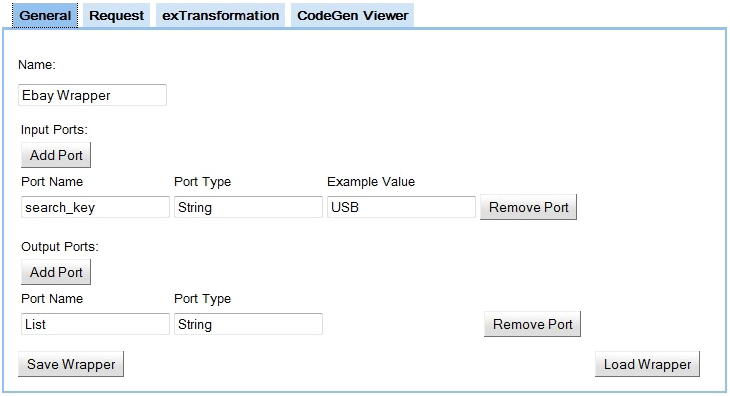
\includegraphics[width=\linewidth]{images/ServiceWrapperToolGVSWithPortDefinitions.png}
    \caption{Configuring parameters of a service wrapper}
    \label{fig:construct_pre_post_conditions}
  \end{center}
\end{figure}

% The service wrapper tool composes the request using a template string which will contain placeholders for input values. Before sending the request to the service, the placeholders are replaced with their corresponding values and the resulting URL is then ready to be sent as the service request.

An example of service request construction can be found in the Figure~\ref{fig:construct_service_request}. In the top input field the user may drop an example HTTP request, taken e.g. from the service's documentation\footnote{\url{http://developer.ebay.com/products/shopping/}}. The tool analyses the example request and in the middle of the screen a form for editing the request parameters is provided. In our example, the user has connected the \textit{QueryKeywords} parameter with the input parameter \textit{search\_key} by adding a corresponding reference to the value field of that parameter. In addition, we have retrieved an access key which has been entered as value for the \textit{appid} parameter.

\begin{figure}
  \begin{center}
    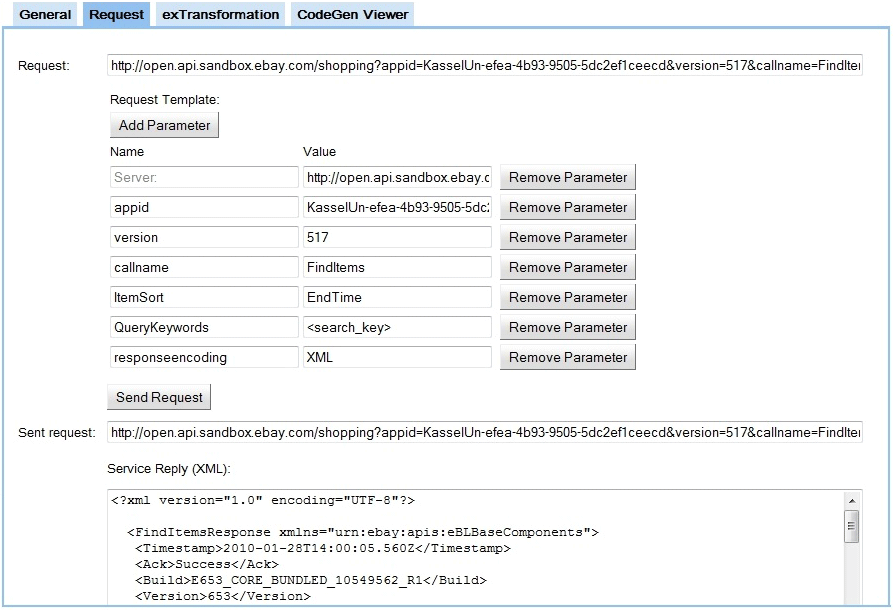
\includegraphics[width=\linewidth]{images/ServiceWrapperToolGVSWithRequestExample.png}
    \caption{Constructing the service request URL and its parameters}
    \label{fig:construct_service_request}
  \end{center}
\end{figure}

Below the request parameter editing form of Figure~\ref{fig:construct_service_request}, a \textit{Send Request} button allows to validate the constructed URL by sending it to the specified service address (via a server relay). 
The service's response is shown on the bottom of the page. This gives the user a fast feedback whether the constructed request works as desired. 

\subsubsection{Limitations} % (fold)
\label{ssub:limitations}

It is worth pointing out that currently the wrapper tool is able to construct input ports for the wrappers using just basic types. To construct URL requests from more complex input parameters, as e.g. a person object, we are currently developing access operations that will allow to access the values of fields of complex objects. For example, the expression \emph{customer.address} may refer to the \emph{address} field of a \emph{customer} parameter.  

% subsubsection limitations (end)

% subsection constructing_service_requests (end)

\subsection{Interpreting Service Responses} % (fold)
\label{sub:interpreting_service_responses}

A web service can choose to send a response message in any desired structured format. In our example, we assume an XML tree, but a JSON structure is equally possible.

\subsubsection{Translation of the Response Tree into Facts} % (fold)
\label{ssub:translation_xml_into_facts}

\begin{figure}
  \begin{center}
    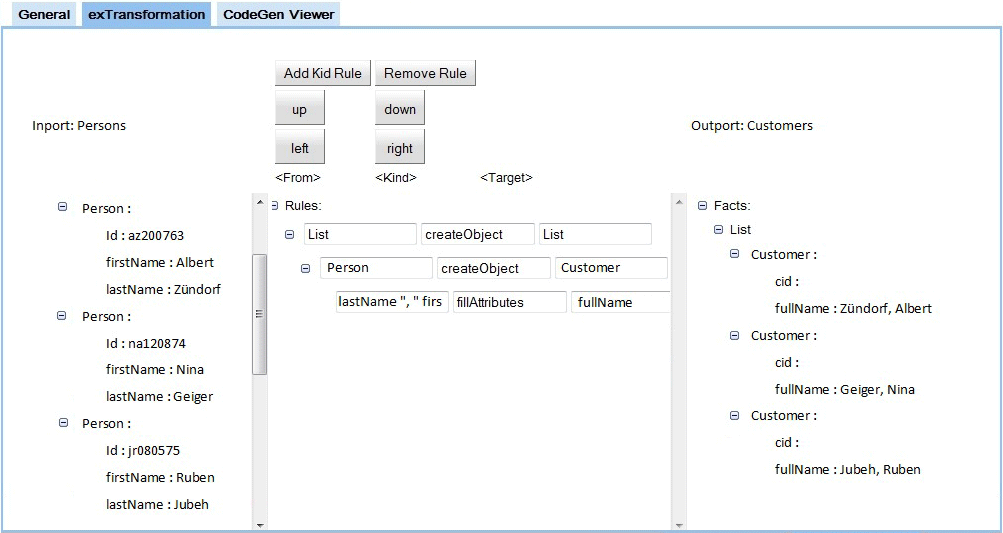
\includegraphics[width=\linewidth]{images/ServiceWrapperToolGVSWithTransformationRules.png}
    \caption{Interactive, rule based transforming of an XML response to domain objects}
    \label{fig:response_service_execution}
  \end{center}
\end{figure}

Once the service response has been retrieved, the transformation tab of the wrapper tool shows it as an interactive object tree, as seen on the left side of Fig.~\ref{fig:response_service_execution}. 

A transformation rule is used to analyse the response data and to generate domain-specific objects from concepts from the ontologies used by the parameters of the different building blocks. A transformation rule is composed of three elements, as seen in the middle part of Fig.~\ref{fig:response_service_execution}. First, the \textit{from} field indicates the source elements to be translated by the rule. Second, the type of the rule will be set, taking one of the following values: \emph{createObject}, \emph{fillAttributes} or \emph{dummy}. And third, the target of the rule specifies a certain concept or attribute, to be created or filled. A detailed explanation of the type of actions to be trigger from the transformation rules is as follows:

\paragraph{createObject} % (fold)
\label{par:createobject}

specifies the creation of a new domain object. The type of that new object is provided in the third compartment. In the example being explained, the root rule searches for XML elements with tag name \emph{FindItemsResponse} and for each such element a \emph{List} object is created. The resulting objects are shown in a facts tree in the right of Figure ~\ref{fig:response_service_execution}.

% paragraph createobject (end)

\paragraph{fillAttributes} % (fold)
\label{par:fillattributes}

does not create a new object but it fills the value of the attribute provided as third part of such rules. In our example, the third transformation rule searches for XML elements with tag name \emph{Title}. Note, the rule is a sub-rule of the second rule, which generates \emph{Product} objects. Thus, the sub-rule searches for \emph{Title} tags only in the subtree of the XML data that has been identified by an application of the parent rule before. For example, the \emph{Item} rule may just have been applied to the first \emph{Item} element of the XML data. Then, the \emph{Title} rule is applied only to the first \emph{Item} sub-tree of the XML data and thus it will find only one \emph{Title} element in that sub-tree (not visible in Figure ~\ref{fig:response_service_execution} ). The value of that \emph{Title} element is then transfered to the \emph{productName} attribute of the corresponding \emph{Product} object.

% paragraph fillattributes (end)

\paragraph{dummy} % (fold)
\label{par:dummy}

does not create or modify any objects but such rules are just used to narrow the search space for their sub-rules. For example, in Amazon product data, the XML data for an item contains sections for \emph{minimum price}, \emph{maximum price}, and \emph{average price}. Each such section contains the \emph{plain price} and the \emph{formatted price}. Thus, in the Amazon case, a rule that searches for \emph{formatted price} elements within an \emph{Item} element would retrieve three matches. Using a dummy rule, we may first search for \emph{minimum price} elements and then search for \emph{formatted price} elements within that sub-tree.

% paragraph dummy (end)

Our tool follows an interactive paradigm. Therefore, any time a change to a transformation rule is done, the transformation process is triggered and the resulting facts tree is directly shown. This process helps the user to deal with the slightly complex semantics of the transformation rules avoiding errors or mistakes. In addition, our tool is ontology-driven, therefore the service wrapper designer retrieves the domain-specific types from a backend server (such as the catalogue discussed in Section~\ref{sec:discovery}) together with the structure of each type, i.e. together with a description of the attributes of each object. Thus, the transformation rule editor is able to provide selection boxes for the target element of the rules. For a \emph{createObject} rule, this selection box shows the object types available for that domain. For the \emph{fillAttributes} rules, the selection box shows the attributes of the object type chosen in the parent rule. 
% In addition, we may provide some analysis tool, which will help to guarantee that the objects generated by the transformation rules conform to the object types defined in the corresponding conceptual model (see Section~\ref{ssec:ontology}). This helps to ensure that the objects generated by the designed service wrapper will be compatible for input parameters of subsequent filter steps and or gadgets.

% subsubsection translation_xml_into_facts (end)

% subsection interpreting_service_responses (end)

\subsection{Generating a Resource Adapter} % (fold)
\label{sub:generating_a_resource_adapter}

Once the wrapping of a service has been defined and tested in the service wrapper tool, we generate an implementation of the desired Resource Adapter in XML, HTML, and JavaScript, ready to be deployed and executed inside a web gadget. 

% subsection generating_a_resource_adapter (end)

\subsection{Limitations} % (fold)
\label{sub:limitations}

The rule driven approach presented above is somewhat limited. It is deliberately restricted to such a simple rule mechanism in order to keep things simple enough for end-users. Still, the selected approach suffices for many practical and real world cases. As a more complex example, the XML data for a person may provide two different tags for the first and the last name of a person. Contrarily, a person fact which conforms to a certain ontology for that domain may provide only one \emph{fullname} attribute that shall be filled by a concatenation of the first and the last name. To achieve this, the \textit{from} field of that transformation rule might look like: \texttt{lastname"', "`firstname}. We are also able to do some navigation in the XML tree to follow XRef elements. For example the attribute \texttt{grandmother} could be filled using \texttt{mother.mother} in the \textit{from} field. 

However, there are some transformations that these rules cannot perform. For example, we do not support any mathematical operations. Thus, transforming e.g. Fahrenheit into Celsius temperatures is not supported. To cover such  cases, intermediate object formats can be used which would allow generating objects to be further processed by additional filters. Such additional filters may be realised using (hand coded) operators, since some generic operators can act as filters for aggregation and conversions of objects from multiple sources. Then, service wrappers in combination with these filter operators will allow covering these complex cases.

% subsection limitations (end)

% section restful_web_services_wrapper_tool (end)